%%%% MACRO DEFINITION %%%%

\providecommand{\pvivax}{P.~vivax}
\providecommand{\pfalciparum}{P.~falciparum}
\providecommand{\cterm}{C-terminus}
\providecommand{\nterm}{N-terminus}

\providecommand{\e}[1]{\ensuremath{\times 10^{#1}}}
\newcolumntype{P}[1]{>{\centering\arraybackslash}p{#1}}
\newcolumntype{M}[1]{>{\centering\arraybackslash}m{#1}}

\providecommand{\refimage}[1]{\figurename~\ref{fig:#1}}

%TC:macro \note [ignore]



%%%%%%%%%%%%%%%%%%%%%%%%%%%%%%%%%%%%%%%%%%%%%%%%%%%%%%%%%%%%%%%%%%%%%%%%%%%%%%%%%%%%%%%%%%%%%%%%%%%%%%%%%%%%%%%%%%%%%
%%%%%%%%%%%%%%%%%%%%%%%%%%%%%%%%%%%%%%%%%%%%%%%%%%%%%%%%%%%%%%%%%%%%%%%%%%%%%%%%%%%%%%%%%%%%%%%%%%%%%%%%%%%%%%%%%%%%%
%													BEGIN
%%%%%%%%%%%%%%%%%%%%%%%%%%%%%%%%%%%%%%%%%%%%%%%%%%%%%%%%%%%%%%%%%%%%%%%%%%%%%%%%%%%%%%%%%%%%%%%%%%%%%%%%%%%%%%%%%%%%%
%%%%%%%%%%%%%%%%%%%%%%%%%%%%%%%%%%%%%%%%%%%%%%%%%%%%%%%%%%%%%%%%%%%%%%%%%%%%%%%%%%%%%%%%%%%%%%%%%%%%%%%%%%%%%%%%%%%%%

\chapter{Computational Techniques} % Write in your own chapter title
\label{Chapter2}
\lhead{Chapter 2. \emph{Computational Techniques}} % Write in your own chapter title to set the page header
In this chapter, the pre-existing algorithms and other computational techniques used to predict Zinc Binding Sites will be outlined.

It will not provide details of specific implementations of them used in this project, or any novel tecnhniques developed - those will be presented in later chapters. It is instead meant to give a general mathematical background to these techniques, and familiarise the reader with the terms that will be used in later chapters.

\section{Machine Learning}

\subsection{Principles}

This project aims ultimately to create a predictor - something which can take either a protein structure or a protein sequence, and determine where, if anywhere, are zinc binding regions.

Machine learning is the use of existing data to create predictive models that can take new data and make inferences about it. It `learns' the characteristics of the existing dataset and uses this to predict certain things about the new data. This can be `unsupervised', where the model simply identifies the internal structure of the data and creates clusters from it, or it can be `supervised', where the existing data is labeled with some correct output, and the model learns how to predict the output based on the input characteristics. If the output is a discrete category, this is classification; if it is a continuous value, this is regression. This is illustrated in Figure ~\ref{fig:machine-learning}.

\begin{figure}
\centering
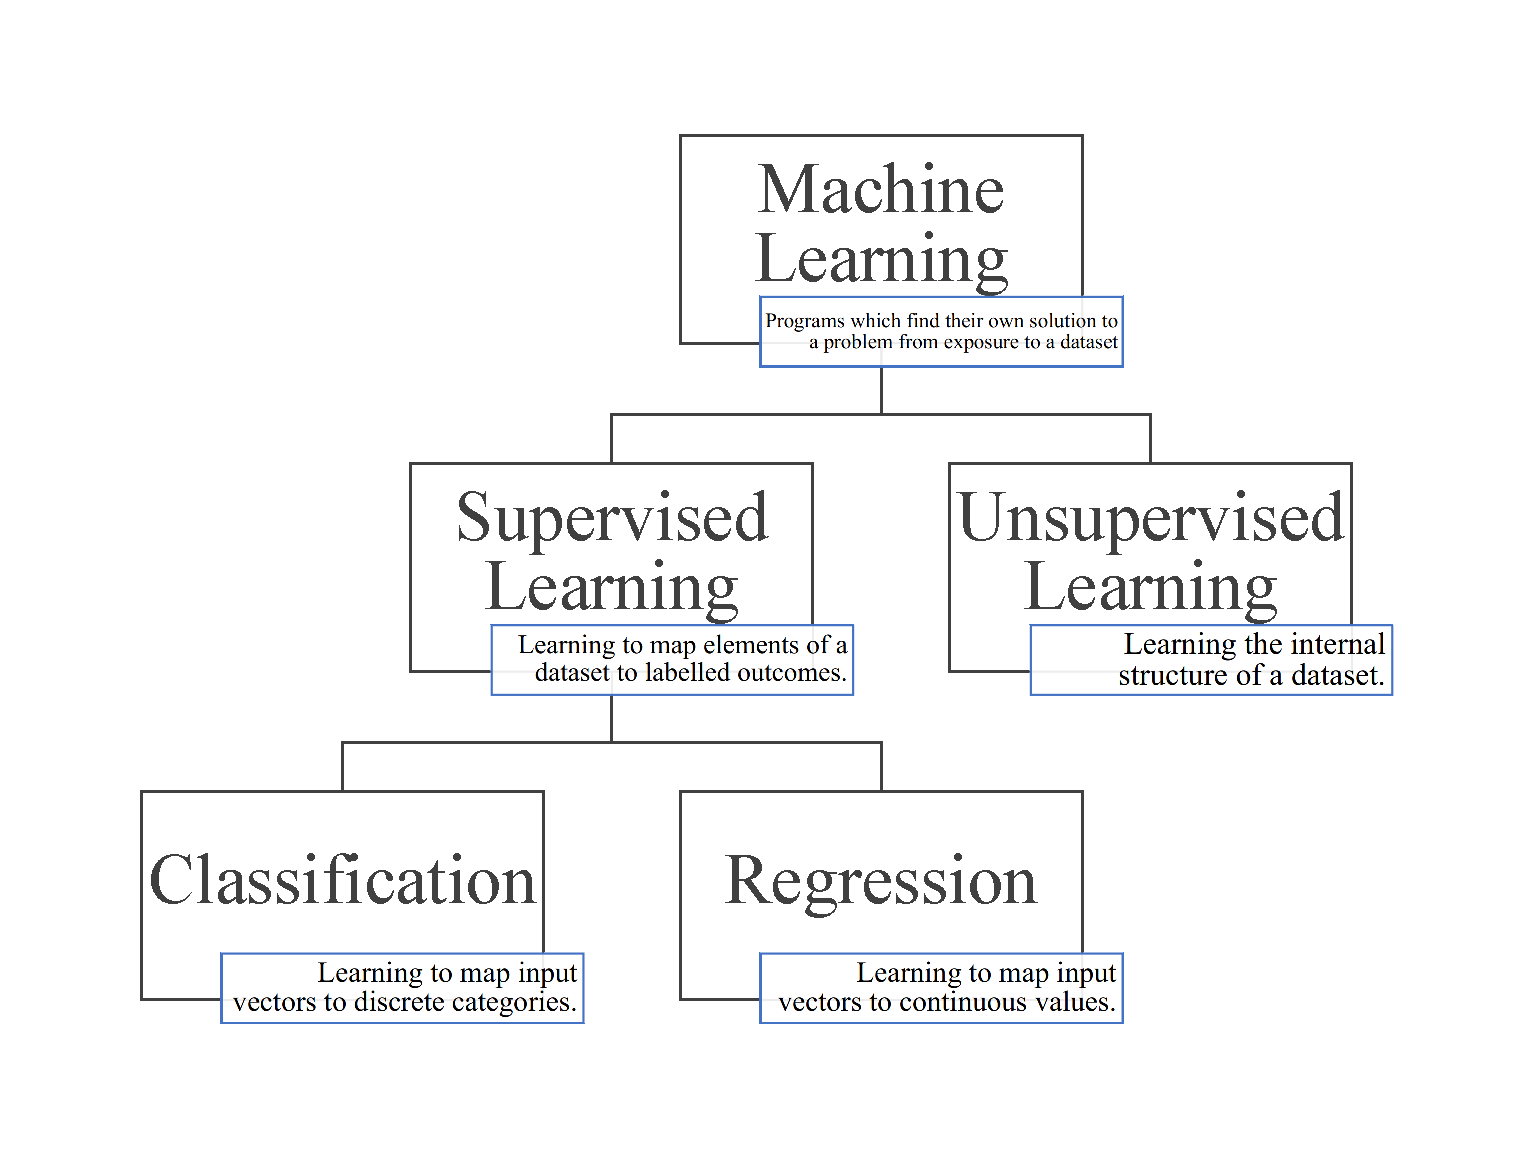
\includegraphics[width=1.0\textwidth]{Figures/machine-learning.eps}
\caption{\label{fig:machine-learning} Overview of the branches of machine learning.}
\end{figure}

This project will use supervised learning, because the dataset being used to train the models will already have the locations of zinc binding sites labeled. 


When the inputs are passed to the model, they are done so as a set of `features'. These are numerical characteristics that the model actually uses to learn what kinds of input belong in which category. These are usually passed to the model as a vector of numbers - classification is just the mapping of vectors to discrete classes, for example. Machine learning algorithms are ultimately mathematical functions, which cannot take in abstract concepts such as `zinc binding residues' as inputs - anything which they accept must be turned into some numerical representation by making numerical measurements of it --- this is its `representation. How the inputs are actually represented is determined by feature selection --- the choice of featyres --- which must be carried out first.

Once the dataset has been processed, models must be `trained' --- a process which varies from algorithm to algorithm, but which is the process by which the algorithm changes its internal workings to perform best on the problem it is given. It is given a dataset to learn from, which in the case of supervised learning is a list of examples of the type of object under consideration, each labelled with the outcome that the algorithm must try and learn. Training here, in the general sense, is the process by which the alogrith learns to develop rules that use the information given for each object to predict the output.

The simplest approach would be to give the model the entire dataset and let it learn from that. However, this can lead to a problem called overfitting, where the model learns details of the training set that are irrelevant - it learns the training set, but is not generalisable to objects not in the training set. To overcome this, the dataset is generally split into a training set and test set, with the latter being held in reserve to assess the model after it has been trained on the training set. If the model is overfit, it will perform much worse on the test set than the training set - if not, the performance on each will be broadly equivalent. By comparing performance between the two, you can measure the extent to which a trained model is generalisable to new inputs it has not `seen' before.

\subsection{Supervised Learning Algorithms}

Supervised learning is the process by which a system learns to map input vectors representing the measurements of some object to discrete output categories, based on the values of those input vectors. However, there are multiple methods and algorithms for doing this. Each of them is suited for different kinds of problem, and they will be outlined here.

The most basic machine learning algorithm tries to find the parameters to some function of the input values, and then finds a threshold above which the positive class should be predicted. For example, some of the earliest methods to be developed were the Perceptron and Adaptive Linear Unit. These create a linear function, with parameters that are learned during training. In this case `learning' means that the output of this function is evaluated for every input in the training set, the sum of the squared errors is found (which acts as a score of how poorly the model has performed with its current parameters), and the derivative of this squared error function is used to change the values of the parameters using gradient descent. Gradient descent is a common optimisation algorithm that tries to find the minimum of a function - sum of squared errors as a function of input vector, in this case. In practice, a variant of gradient descent called stochastic gradient descent is generally preferred, where a random subset of the training data is used each time. This speeds up the rate of optimisation and allows the function to escape local minima.

Linear perceptrons are relatively primitive - they use a linear function and so can only separate data that is linearly separable in the first place, meaning that a line, or plane (etc.) can divide the data in space. However they do illustrate many of the principles that are common to most or all supervised learning algorithms. Many of them have the overall architecture of a function with learned parameters and a threshold, for example. They also illustrate the difference between parameters and `hyperparameters'. A parameter is something the algorithm itself learns, and in this case the parameters are the coefficients of the linear equation, and the threshold value. So for n-dimensional input vectors, there will be n + 1 parameters to learn. A hyperparameter on the other hand is a `setting' that the user manually sets. For example, the number of passes through the data to make (epochs).

A more sophisticated variant of the perceptron is a supervised learning algorithm called logistic regression. In logistic regression, you still have a linear function whose coefficients the system tries to learn using (usually stochastic) gradient descent. However in this algorithm, before checking the output of the function against a threshold, the value is passed into a second `activation function' which is not linear. In this case the activation function is a sigmoid-like function that maps all inputs to some value between -1 and 1.

Support Vector Machines (SVMs) are another variant of the basic perceptron model which is widely used in classifcation tasks. In this case, the learning algorithm is iterated until the distance between the closest input vectors to the decision boundary (the support vectors) is maximised --- an extra consideration that increases the cleanness of separation between the categories.

Not all classification algorithms take this form of fitting the parameters of a function and then applying a threshold cutoff.

Decision trees, for example, divide the input space into regions by a series of branching cutoffs. At the first `node', a dimension and a value which maximally separates the categories is picked, bifurcating into two branches. For each of these two branches, another bifurcation takes place, and so on until the categories are separated. The number of nodes - the depth - is a hyperparameter that is chosen beforehand. This can be a very important consideration - too few nodes, and the algorithm will usually not be able to cleanly separate the data, with low recall and/or precision being achieved. However if there are too many branches, the model will become overfit - it may perfectly separate the training data, but in doing so will learn statistical noise present only in that sample, reducing its ability to generalise.

The metric that decision tree algorithms use to identify how to bifurcate is entropy, a measure of uncertainty in this case. At each bifucation point the algorothm must select a feature and a cutoff value for that feature, and it does so based on the combination that would best split the two output categories under consideration (i.e. the combination that would most reduce entropy).

An extension of the decision tree that can be very effective is the random forest classifier. This algorithm generates multiple decision trees (the precise number being a tunable hyperparameter), each of which is trained on a random subset of the available training data. When a new input is to be classified, each of the trees classifies it according to its own training, and a majority vote is taken to determine the forest's verdict as a whole. This is an example of `bagging' (bootstrap aggregating), where the noise and errors of individual models are canceled out in an averaging.

Another supervised learning classification algorithm is K-Nearest Neighbours. This is a slightly unusual algorithm as it has no parameters that are tuned during training. Instead `training' in this case simply means giving it the entire training dataset, which it stores, and this entire dataset is used when classifying new inputs. The k closest vectors in the training set to the input to be classified (the k nearest neighbours) and identified using some distance metric (typically standard Euclidian distance) and a majority vote is taken - the category most represented in the nearest neighbours is the predicted category for the input. The main hyperparameter for this algorithm is the value of k - the number of neighbours to look for. An odd number is usually preferable, so that for binary classification problems there will always be a winner of the majority vote.

K-Nearest Neighbours illustrates a problem that is present in many machine learning algorithms - the so-called `curse of dimensionality'. That is - the more dimensions a dataset has, the harder it is to create effective, predictive models. This is not just because of the extra computational burden. Higher dimensional data is more `sparse' - the distances between objects gets larger. In the case of K-Nearest Neighbours this can be a problem because the nearest neighbours are further away, and the distance of the nearest neighbours approaches the average distance between data points as dimensionality increases, reducing the information content in those neighbours.

The above supervised learning methods are established algorithms for classifying inputs into categories using single functions. They are widely used, and have been used with considerable success in bioinformatics problems - including the identification of zinc and other metal binding sites (see below). However, there are limits to the discriminatory power of a single function, linear or otherwise, and hence limits to the complexity of the underlying system they can model. Their `capacity' - the space of possible functions they can assume to model reality - is limited.

Rather than utilising a single function, deep learning uses nested functions - each with its own set of parameters - to capture different layers of abstraction in the input data. There is an input layer, which maps the input vector to some intermediate vector which represents some aspect of the input data. One or more hidden layers then acts on these intermediate vectors, eventually passing the data to the output layer which produces a vector representing the model's degree of certainty that the input belongs to each of the possible categories. Each layer acts as a kind of perceptron with a non-linear activation function - if they were all linear then the model as a whole would be linear. This architecture is a neural network, and this is the classical implementation, with every layer fully connected to the layer before it.

Training a neural network requires finding the optimal values for the weights and threshold for each layer. Using the usual technique of defining a cost function and the differentiating this over the various layers would be very computationally difficult to do with the necessary precision. Fortunately a shortcut exists called backpropagation, which allows the neural network to be trained with much fewer computational resources.

There are variants of the artificial neural network (ANN) model outlined above which are better served for different kinds of tasks. Convolutional Neural Networks (CNNs) are a widely used variant that are optimised for processing images and other input spaces that can be thought of as regularly spaced grids in n dimensions. Rather than having every layer fully connected to the layer before it, there are a number of `convolutional' layers in which the perceptrons only connect corresponding localised regions - followed by normal fully connected layers at the end. Rather than standard matrix multiplication, a mathematical operation called convolution is used to determine the forward flow of information through the network.

Another variant is the Recurrent Neural Network (RNN). In standard neural networks, the input data is unordered, and each input is treated in isolation - the network `forgets' what it has just done and treats each input like it was the first. However often datasets have inherent order, and knowledge of what the last input was classified as (or what the last n classifications were) contains important, usable information for classifying the current input. Recurrent neural networks are usually used for sequential data therefore, and are therefore of use in dealing with biological sequences (see below). They operate by adding an extra term relating to previously classified inputs.

Deep Learning is a kind of representational learning - the model itself is learning the features in the input space that are important. This can be seen when processing images - the model's first layer may look for low-level properties of the image, such as regions of high contrast representing borders, the next layer may look at simple combinations of these, and later layers will be sensitive to more high level combinations of visual features. This is inspired by - though does not work in precisely the same way as - the mammalian visual cortex.

\subsection{Evaluation}

A trained model will (in this case) map potential binding sites to one of two categories --- zinc binding or not zinc binding. To determine how useful a model is, or if it still needs improving, there needs to be a measure of how well the model is performing. There are a number of metrics for determining classification model performance.

To evaluate the model, a number of test inputs are given to the model, and for this purpose, the model can produce one of two outcomes, true or false, so all of the test results fall into one of four categories - true positives (correctly identified as a binding site), false negatives (was a binding site, but not detected), false positives (not actually a binding site, but wrongly identified as one), and true negatives (not a binding site, not identified as one). The first and last categories are the ones we want to optimise for, the other two the errors.

The simplest means of grading a model is with accuracy - the total number of correct predictions (true positives and true negatives) as a proportion of all test inputs. This can be a misleading metric however, if the dataset is class-imbalanced - that is, if one class is much more prevalent than the others. This will be the case in this project, as non-zinc binding regions vastly outnumber zinc binding regions. Accuracy is misleading here, because a model which just always predicts the more-prevalent class can get a very high accuracy, despite being completely useless as an identifier of rare states.

$\mbox{accuracy} = \frac{TP + TN}{TP + FP + FN + TN}$

Similarly the error rate - the total number of incorrect predictions (false negatives and false positives) as a proportion of all assignments - suffers from the same problem, and should be treated with the same caution in a class-imbalanced problem like this.

Two more meaningful metrics are precision and recall. Precision is the number of true positives, as a proportion of all predicted positives - that is, how many positive predictions were correct? Recall (also referred to as sensitivity) is the inverse, the number of true positives, as a proportion of all actual positives - that is, how many actual positives were identified? A high precision means that false positives are being kept down, with the reported positive cases being mostly correct. A high recall means that false negatives are being kept down, with most of the positive cases being identified.

$\mbox{precision} = \frac{TP}{TP + FP}$

$\mbox{recall} = \frac{TP}{TP + FN}$

However these two metrics exist in a balance, with improvements in one causing a decline in the other. The more `eager' the model is to assign a positive prediction to an input, the more of them will be identified and the higher recall will be - but a smaller proportion of the predicted positives will be correct, lowering precision. Likewise, the more resistant the model is to predictive a positive label, the higher precision will be, but the lower recall will be.

Another important metric is specificity, often contrasted with recall/sensitivity. This is the proportion of inputs the model reports as negative which are actually negative, and is a measure of the model's ability to correctly ignore negatives.

Usually it is convenient to have a single value representing the effectiveness of the model, which is done using the F1 Score. This is simply the `harmonic average' of precision and recall - the ratio of their product and sum, multiplied by two.

Another single value measure of model effectiveness is the Matthew's Correlation Coefficient, or MCC. This takes into account all four values in the confusion matrix, and has certain advantages over the F1 score in that it ``produces a high score only if the prediction obtained good results in all of the four confusion matrix categories" \cite{chicco2020mcc}.

$\mbox{MCC} = \frac{TP \cdot TN - FP \cdot FN}{\sqrt{(TP + FP) \cdot (TP + FN) \cdot (TN + FP) \cdot (TN + FN)}}$

There are metrics which show not how effective the model is in its current state, but how its ability to distinguish one class from another varies over different thresholds. Most classification algorithms can assign a probability of being in one class or the other, and the actual prediction is made by setting some threshold - if the probability is above this threshold, the positive case is predicted. If not, the negative case is predicted. A ROC Curve will show the model's effectiveness changes as this threshold is changed, by plotting false positive rate against true positive rate for every threshold value (to some given resolution). Purely random classifiers will produce a diagonal line - as the threshold is increased, both true positive predictions and false positive predictions will increase by equal amounts because the model can't actually distinguish one class from another at all. The better the model is at making this distinction however, the more this line will curve into the top-left corner, because true positives will increase much faster than false positives in a `good' model.

This graphical ROC curve can be represented in a single metric called the AUC - area under the curve. As the name suggests, this is the area underneath the ROC curve, which will be 0.5 for a purely random model, and 1 for a perfect model. The reason a perfect model has an AUC of 1, is because a perfect model will have some threshold which produces a true positive rate of 1 and a false positive rate of 0, meaning it will touch the top left corner of the plot. Again this is a measure of how easy it is for the model to separate the two classes.

Another means of evaluating a model is examine how its performance increases with increases in training set size --- learning curves. In this analysis, the model is trained in random subsets of the training data of increasing size, and the training and test scores taken at each stage --- the score used depends on what is being assessed. This is useful in assessing the rate of convergence (how the model's training performance is approaching the test performance) and in determining whether a model would benefit from more training data.

Another pair of properties of models that is important to monitor is their bias and variance. These are both measures of the inadequacy of the model, but represent different things. A model's bias is the error that results from it making incorrect assumptions about the thing being modeled --- it might be too simplistic for example. Variance by contrast is error caused by being too sensitive to the specific data points used to train it.

This is related to the concepts of underfitting and overfitting respectively. A model which is underfit does not have enough parameters to properly represent the function it is modeling, and a model that is overfit is too attuned to the training data, which is after all only a sample. An overfit model will perform very well on the data it was trained with, but poorly on inputs it hasn't seen before --- it has `learned its training set.' A common way around this is to train the model on a subset of the available data --- typically around 80\% --- and then measure the model's performance on the remaining test set. 

Any measures taken to reduce overfitting are called regularisation. These include general best practices, such as the previously mentioned practice of evaluating a model on a different dataset from the one used to train it, as well as algorithm specific measures, such as (in the case of Decision Trees/Random Forests) reducing the number of splits the tree is allowed to make.

Machine learning has been successfully applied to many areas of Bioinformatics in recent decades, with particular successes in the recent decade. It has been used for the specific application of predicting zinc and other metal binding sites since there was enough data to construct the initial minimal datasets in the 2000s, and it is worth reviewing the progress that has been made here.

\section{Machine Learning to Predict Zinc Binding}

There are still many proteins whose function is unknown. In many cases we only know their sequence, though some of these have had their structure solved experimentally. One means of determining what function a protein might be intended to perform is to look for certain proerties associated with a given function in already charactersied proteins, and then look for these properties in uncharacterised proteins. If, for example, it can be shown that such a protein had one or more zinc binding sites, that could offer insights into what function the protein performs. Indeed, that is ultimately the goal of this project.

Owing to this clear usefulness, there have been a number of attempts to develop such predictors in the past, dating back to the early 1990s. These methods and techniques form the essential context in which my own project should be understood, and also provide the benchmark of success against which my methods should be judged. Here their progress will be reviewed. They can essentially be divided into two broad categories - prediction from structure and prediction from sequence.

\subsection{Prediction from Structure}

Predicting zinc binding from structure takes the atom coordinates of some protein as its input, and produces as output residues in that structure which are believed to be able to bind zinc if zinc were present - generally along with some estimated probability that this should be the case.

This is perhaps of only limited utility, as very often proteins which can bind zinc tightly will have zinc bound when the structure is solved, and so no prediction is required. Where such methods are of use however is when a protein capable of binding zinc is crystallised without zinc being present - presumably because the researchers didn't know it could bind zinc and so did not provide any in the medium. These apoproteins can be scanned by predictors like this to identify unfilled zinc binding sites.

The earliest attempt at a general purpose prediction algorithm was the Hydrophobic Contrast Function, developed in 1990 \cite{yamashita1990metal} to detect metal binding sites in general. This began from the observation that metal atoms tended to be surrounded by a shell of hydrophilic atoms, which in turn were surrounded by an outer shell of hydrophobic atoms. They developed a function which took as its input a coordinate in space, and returned a measure of this `hydrophobic contrast' at that location. They showed that by scanning every point in the structure on a grid, evaluating the function at every point, and then ranking the points by their score (the function returned values between -1 for inverted contrast and 1 for desired contrast), the highest scoring points would be clustered at sites of metal binding.

This was the first demonstration that a property of metal binding sites could be used to create a predictive model. However it should be noted that it was only tested on structures with metals already present, not on apoproteins, and the initial observation itself was based on a very small number of metal proteins that were available at that time. It was later expanded upon by combining it with a template-based searching algorithm, whereby the known metal binding sites were represented as stripped-down `templates' of just alpha and beta carbons, and used to search proteins using a simple pattern matching algorithm \cite{gregory1993prediction}. Once a set of three residues matching a known template was found, the hydrophobic contrast function was applied to verify that the binding site was a region of high contrast, which it generally was. This was part of a pipeline for engineering binding sites into proteins, so it didn't require the matching residues to be of any particular type, but the general principle of using known site geometry and hydrophobic contrast properties to look in new structures was still in use.

The use of physical properties such as hydrophobicity has in some cases been taken to the logical extreme through the use of molecular dynamics, and the full-scale modeling of the interactions between protein residues and a hypothetical metal atom and the use of empirical force fields which can describe the attraction that a small molecule should experience towards a region of a protein. However, the standard force fields developed for molecular dynamics tend not to model metal-protein interactions well, so specific force fields for this branch of chemistry need to be developed. One such force field, the Fold-X empirical force field, was adapted for use on single atom ligands such as water and metal atoms \cite{schymkowitz2005}. Not only were they able to `decorate' protein surfaces with identified metal binding sites, but the implied affinity of the binding sites reported by the force field correlated closely with experimentally reported affinities where available.

Generally however, many systems for predicting zinc binding in structures use geometric searches of some kind -- particularly the early attempts. In 1997 a database of `structural motifs' was built, as well as a simple algorithm for searching a structure for them called TESS (Template Search and Superposition Algorithm) which used hash tables for fast lookup \cite{wallace1997tess}. While not specifically targeted at finding metal binding sites, the small structural motifs that it specialised in are particularly applicable to small ligand binding sites.

Simple geometric templates were eventually used to specifically identify metal binding sites again in the 2000s. Calcium binding sites have been successfully predicted by simply looking for clusters of oxygen atoms and identifying their centre \cite{deng2006} for example. In 2008, Goyal and Mande built up more complex templates using pairs of residues to identify previously unknown sites --- from a now much larger starting dataset of structures. While this attempt was a general purpose metal binding site predictor, it was largely trained on zinc binding sites as they found that all metal binding sites had broadly similar geometric distributions of alpha and beta carbons. This observation is important in distinguishing zinc binding sites from other metal binding sites.

One of the first template-based tehcniques which looked at zinc binding sites specifically was the TEMSP method, developed in 2011 \cite{zhao2011structure}. Here again the problem is simplified by creating a library of `residue pairs', where for each zinc binding site obtained from the PDB, they store each pairwise combination of liganding residues (actually just certain properties of them, such as alpha-alpha distance etc.) and then search the target protein for these. Once one is found, other template pairs are superimposed on the structure to find additional liganding residues. They used a stricter definition of `true positive' than previous attempts, and still reported a sensitivity of 86.0\% and a selectivity of 95.9\% in their test dataset - barely lower than the values obtained when testing on the training dataset used to refine their parameters. When applying their tool to a dataset of proteins of unknown function, they found some very promising results - finding 186 probable zinc binding sites. Unfortunately, the online version of this tool is no longer accessible at time of writing.

The use of geometric techniques to identify both zinc and other metal binding sites has continued up until the present day, despite the increase in interest in more complicated machine and deep learning techniques over the 2010s. In 2013 a straightforward database survey of high quality zinc binding proteins (low resolution, high occupancy, low B-values) produced geometric templates that identified zinc binding sites at rates comparable with other methods --- though like many of those other methods they restricted themselves to sites made of the four common residues cysteine, histidine, aspartate and glutamate, the CHED residues \cite{liu2014}. The ubiquity of these residues inspired the name of a similar tool around this called CHED, which again relied on geometric templates to predict zinc binding sites specifically --- though with an extra filtering step for removing false positives \cite{sobolev2013web}.

As has been noted, while much attention has been paid to predicting whether a region of a protein binds zinc or some other metal, discriminating which metal binds to a region of a protein known to bind a metal is less well studied, and not straightforward owing to the similar preferences that transition metals tend to have in terms of the geometry, distance and chemical nature of their liganding atoms. A geometric approach was used here in 2015 with the algorithm mFASD, which examines the atoms in contact with the metal centre to create a `functional atom set`, creates a library of known functional atom sets for particular metals, and determines the set's `distance' (not Euclidian distance, but rather a measure of the difference between two data structures) from each characteristic set --- the functional atom set distance (FASD) \cite{he2015}. Using just this information they were able to get AUC scores ranging from 90\% and 50\%, depending on the metal pair in question, and demosntarted the feasability of distinguishing the binding sites of different metals. 

The most recent purely geometric approach to predicting metal binding is from 2019, which uses known metal geometry rules rather than a survey of known protein structures particularly \cite{sciortino2019}. Their method, called GaudiMM, is notable in that after making the side chains in the test set `flexible', their success rate only slightly decreased - an important property of any system that proposes to find metal binding sites in apoprotein structures.

The research outlined above did not use machine learning techniques, but rather simple geometric templates and other rules based on observed properties of zinc and other metal binding sites in proteins. What distinguishes them from those which do use machine learning is not the use of geometry as such --- geometric attributes are often part of the featureset fed to machine learning algorithms --- but rather the use of a human to determine what features to pay attention to. Machine learning algorithms by contrast, while they vary widely in implementation details, are generally left to determine by themselves what features are important and how to use the data given to them to classify objects.


MetSite was one of the earliest use of machine learning techniques to predict binding sites as we would use the term today, in 2004 \cite{sodhi2004predicting}. They used artificial neural networks to detect metal binding sites in low-resolution structural models, such as those generated computationally from sequence data. They set themselves a target of having a false positive rate no higher than 5\%, and using this threshold were able to get an  accuracy of 94.2\% and, more informatively, a recall of 60\% - across all sites. These figures fall to 84\% and 39\% for specific metals, from which they infer that many metals in the structures used are labelled incorrectly. They show that their model can predict metal binding in proteins of unknown function, and in models generated computationally, because the features they use don't use information from the precise positions of liganding atoms, but from outer residues and secondary structure.

An important development in 2008 showed that decision trees and support vector machines could be used to identify metal binding sites in apo-protein structures - that is, structures solved in the absence of the metal in question \cite{babor2008}. This was an important proof-of-concept as it demonstrated that in the absence of the metal atom, the liganding residues are still sufficnetly close to their liganding conformation to allow them to be identified from atom positions. A similar study in the same year showed that Bayesian classifiers (models which use training dataset to prgressively apply Bayes' rule of probabilistic inference) alone could identify zinc binding sites specifically, using only concentric shells of atoms around the site as features \cite{ebert2008}. This latter paper makes the point that Bayesian classifiers have a distinct advantage over more complex machine learning methods in that the model is less of a black box --- you can follow the decision making of the classifier more easily.

Another use of Random Forest from that same year also produced reasonably encouraging results --- an AUC of 0.8 \cite{bordner2008}. Random Forest is particularly suited to measuring the importance of the features that are given to the model, and in this case they found that accessible surface area and the level of evolutionary conservation of the residues in question were particularly important properties to examine. This was also another example of a model who's efficacy remained largely the same when apostructures were examined. This finding was repeated in a similar piece of research in 2012 \cite{zheng2012}.

There have been uses of deep learning in recent years however, with encouraging results. In 2019 a system in which an ensemble of different classifiers were used as the inputs to a neural network was developed quite successfully --- demonstrating the power of using multiple classifiers trained in different ways \cite{li2019}.


There has also been some attention given to the problem of detecting half binding sites --- regions of a protein chain's surface which would form part of a binding site if another half binding site is present. In 2011 the mutation in the complement factor H protein which causes them aggregate was investigated by a number of experimental means, as well as with a bioinformatics approach \cite{nan2011zinc}. Here the approach was largely one of molecular modeling - creating multiple dimers of the protein in various conformations and looking for arrangements in which there was no steric clash and in which an arrangement of residues is made which could bind zinc (they used METSITE for this). While they didn't find a definitive zinc binding site in this way, they did rule out a site which they had strongly suspected of being responsible beforehand. Note also that this is a search for a full zinc binding site between two specific proteins --- it is not a search for a half binding site on one protein. That is, it relied on knowing what the other `half' of the binding site would be, at least at the whole protein level.

There have also been some purely experimental investigations in this phenomenon, such as the demonstration that zinc mediates the oligomerisation of the Alzheimer's protein Amyloid Precursor Protein, shown through FRET analysis \cite{mayer2014novel}. In general however, the examination of finding half binding sites in protein structures has been very understudied.

\subsection{Prediction from Sequence}

A system for identifying zinc binding residues from the mere sequence of residues it contains is arguably much more useful, as protein sequences are much more readily available. It allows for whole genomes to be scanned for zinc binding proteins. As such, there has been much effort in the past to create techniques for predicting zinc binding from sequence.

The earliest research in this area was largely a `manual' effort, given the small number of sequences available. The discovery of zinc finger proteins in 1985, for example, involved the observation of repeating C...C...H...H patterns in the proteins being studied, and the hypothesis that these were binding zinc \cite{miller1985repetitive}. Similarly, zinc binding in the E6 and E7 subunits of a Papillomavirus was predicted from the observation of cysteine repeats \cite{barbosa1989papillomavirus}. Slightly more complex patterns were later identified, such as the observation that enzymatic zinc binding sites frequently have two residues close to each other in the sequence, and then a third much more distant --- the `short and long spacers` \cite{vallee1989short}. This kind of manual examination of individual protein sequences is obviously not scalable to the vast numbers of protein sequences now available, and can only identify relatively obvious binding sites in any case --- but the same principles that were used in these early studies of characteristic repeats largely underpins the automated techniques now in use.

As the number of sequences grew, identifying zinc binding sites through the use of sequence alignment to known zinc binding sequences became possible. This was used to identify plausible sites in Protein Kinase C \cite{bishop1991identification}, in {\it Giardia lamblia} surface proteins \cite{nash1993variant}, and in the Alzheimer's protein Amyloid Precursor Protein (APP) \cite{bush1993novel}. While this sort of manual inspection for characteristic sequences would largely by sueprceded by more automated methods from the mid 1990s onwards, it is still occasionally a useful feature of research when a single protein is being researched in detail --- being done recently to identify a novel zinc binding protein in yeast from an observed CXXCXXXXXCXXC pattern \cite{furukawa2018identification}.

One of the ultimate advantages of sequence prediction over structure prediction is that it allows you to quickly and efficiently search very large datasets for evidence of zinc binding. Again, early efforts relied on sequence alignment --- in 2004 every then-known metal binding sequence was encoded as a series of residue codes and gap sizes (referred to as `metal binding patterns'), and these were then BLAST searched against entire genomes of various species \cite{andreini2004hint}. The same team would go on to study zinc binding in the human genome specifically using a refined version of this technique and assert, based on this method, that the human genome encodes 2,800 +/- 400 zinc binding proteins --- about 10\% \cite{andreini2006counting}. Shortly afterwards they expanded their analysis to representative genomes from eukaryotes, prokaryotes and archaea, and found that this proportion varies from 4\% to 10\% --- with eukaryotes having more due to higher numbers of regulatory proteins \cite{passerini2007predicting}.

Largely however, as with structural prediction, the bulk of research efforts have focused on the use of machine learning methods. One of the first uses of traditional machine learning methods was in 1995, when neural networks were employed to predict zinc finger proteins from sequence data \cite{nakata1995prediction}. They hardcoded the specific C...C...H...H spacer pattern they were looking for into the model, rather than having the model learn it from existing sequence data by encoding it as a binary feature, and also incorporated features for electric charge, hydrophobicity, and side chain types. Overall this was largely successful - they reported an accuracy of 97\%, though for a very specific type of zinc binding sequence that was largely hardcoded in from the start. Another early use of neural networks to predict metal binding using neural networks was in 2005, when a one-hidden-layer network was used to predict a variety of metal binding sites in sequence \cite{lin2005protein}. Though they did not look at zinc specifically, it, like the previous example, demonstrates that it is possible to build effective models --- with high sensitivity in this case --- from comparatively small amounts of data (at least compared with the volume of sequences available now).

Both SVM and neural networks were used to predict the metal binding cysteine and histidine residues of sequences by the same group that developed the metal binding pattern concept --- though it relies on the sites present in the searched sequence belonging to previously identified motifs, as it is these previously identified patterns that their models were trained with \cite{passerini2006identifying}. They would later extend this to use inter-cysteine distance information \cite{passerini2007predicting}.

Another use of SVM models from the same year reported a sensitivity of 74.9\% and a specificity of 98\% for zinc, using a variety of features, and found that of all the features they looked at, hydrophobicity, solvent accessbility and polarity were the most important features used by the model in prediciting zinc binding from sequence \cite{lin2006prediction}. The combination of raw sequence data with homology modelling was validated using another SVM model in 2008, in a tool called ZincPred \cite{shu2008prediction}. They reported high scores, but should be noted that they had a relatively forgiving metric of success (at least one residue in a binding site correctly identified) and, like many sequence based models, it only predicts at the residue level --- that is, the inputs are individual residues, and the model predicts whether that one residue is metal/zinc binding or not, rather than identifying discrete binding sites. SVM models were widely used throughout the 2010s, most recently in 2018 \cite{srivastava2018prediction}, with broadly similar results.

Random Forest has also been used successfully in the prediction of zinc binding sites from sequence, again relying heavily on Position-Specific Scoring Matrices \cite{zheng2012}, \cite{Kumar2017} --- an advantage of which is the relatively straightforward means of determining which features are the most important in making correct predictions.

And also in keeping with the structural models, the use of ensemble methods --- where multiple models are trained and then vote --- has also been used, in the case of sequences for a model called ZincExplorer \cite{chen2013}. An interesting example of this was in 2017, when three previous zinc binding site predictors --- ZincExplorer, ZincFinder, and ZincPred --- were used to predict zinc binding from sequence, and then the output of these individual models were fed into a novel linear regression model, yielding very high results \cite{li2017}.

In the past couple of years the use of deep learning techniques has begun to have a more pronounced effect on the field. In 2019 an alternative to molecular docking --- where the binding affinity of a ligand and protein is calculated by simulating the correct pose/position of the ligand on the protein, and then calculating the energy of binding from that position --- was proposed called DeepAffinity \cite{karimi2019}. This uses mostly recurrent neural networks to remove the need for these separate steps, and simply predicts affinity as a function of the structure alone.

Other uses of deep learning to predict metal binding from sequences include combining convolutional and recurrent neural networks to predict metal binding histidines and cysteines (which found the mutation rate feature to be most significant) \cite{Haberal2019}, a novel means of representing protein sequence using continuous vectors, which they apply among other things to the task of metal binding site prediction \cite{heinzinger2019}, and a use of a technique called `extreme gradient boosting', which predicts ligand binding sites generally at a similar success rate as previous techniques, but faster \cite{zhao2019}. This is a modification of the gradient boosting algorithm, which has also been used to predict metal binding residues from sequence, albeit largely relying on structural attributes predicted from the sequence \cite{hu2020}.

Machine learning has therefore been used successfully in the prediction of metal binding sites generally and zinc binding sites specifically. One recurring feature that should be pointed out in closing, particularly in the sequence-based
predictive models, is the focus on zinc binding \emph{residues} rather
than zinc binding \emph{sites}. In most cases, the entity examined by the predictive model
is the individual residue, often with a surrounding linear sequence `window'
of residues. The model then assigns a probability as to whether that
residue is a zinc binding residue. As outlined above, this approach has 
had a measure of success, but it is a somewhat artificial
concept. There is, after all, no such thing as a zinc-binding residue
in isolation. The individual residues of a high-affinity zinc binding
site of the kind considered here are only zinc-binding when the other
residues are present, and conversely many non-zinc-binding residues
could bind zinc if other residues were present in the correct
locations. It is particular \emph{combinations} of residues, not individual
residues, which are zinc binding --- an important fact not usually
considered in research of this kind.

Another commonality is the treatment of zinc binding sites as a single
category, and the presumption of properties that are common to them
all regardless of the residues of which they are comprised. This may
well be sufficient --- particularly as there are essentially only four
residues that make up the vast majority of zinc binding sites --- but
it is possible that properties used for prediction have much tighter
distributions within particular sub-categorisations of zinc binding
sites.

These are both crucial issues, which this PhD will attempt to address.

\section{Sequence Techniques}

As part of the dataset generation process, sequence clustering is used. This takes a set of sequences - peptide sequences in this case - and creates a non-redundant set of sequences from them where very similar sequences are grouped together, with a similarity cutoff use to determine which sequences should be considered similar enough to group \note{what does this value represent?}. This has the advantage of ensuring that sequences which are overrepresented aren't given undue weighting in analysis simply because they are present in more copies. The program CD-HIT is used to perform this analysis. \note{Cite.}

BLAST (Basic Local Alignment Search Tool) searching is also used in this project, which is an algorithm for searching through a database of protein (in this case) sequences for those which align to a query sequence. It uses heuristics to perform this search very quickly. It is `local' alignment in the sense that the query is not just aligned to the whole target sequence --- if it has a better alignment with a substring of the sequence, that will also be identified. \note{So what, and cite.}

\section{Web Technologies}

A major part of this project's utility to the wider scientific community is the presentation of the data and tools created for it to the world. All of them are available via the web, and various web technologies are used to accomplish this.

\note{GitHub/Git? Django->Python/Django? React-?Javascript/react?}

\subsection{Django}

Django is an open source Python web framework, used to create database-backed web applications \cite{django}. All database population scripts are written in Python, and use the Django Object-Relational Mapping utilities to populate the database.

\subsection{GraphQL}

GraphQL is an API technology and query language which allows users to construct requests for precisely the data they need - no more, no less \cite{graphql}.

Traditionally, web APIs have used the REST archictecture, whereby every meaningful object is given a URL address. The problem that GraphQL seeks to address with REST is that REST APIs often involve overfetching (you get the full representation of an object whether you want it or not) and underfetching (you have to make multiple requests to get the data you need). With GraphQL APIs, you define your objects using a graph of relationships, and then request exactly the data you need.

GraphQL APIs are used here to provide computational access to both the dataset itself, and to the predictive models.

The Python/django library graphene is used here to implement the GraphQL schemas and API services \cite{graphene}.

\subsection{React}

While the web services provide computational access are useful for programmatic access, for browsing the data initially a website frontend is much more useful. In order to avoid duplication of logic, a JavaScript framework which connects to the existing API is used here - React \cite{react}.

React uses individual components to build up a single page web application, and the React router package is used to create individually addressed pages.

Other JavaScript technologies used on the frontend are the 3D macromolecular visualisation package NGL (used for visualising the zinc binding sites) \cite{rose2015ngl} and the charting library highcharts (used to give an overview of the data) \cite{highcharts}.

\section{Conclusion}

Predicting zinc binding sites is a binary classification task --- all potential sites in a protein, whether that is defined as a location in space or a combination of residues, must be assigned to the category of `true zinc binding site' or `non zinc binding site', using information about what distinguishes these categories from a dataset of confirmed zinc binding sites.

This is a task for which there are a variety of well established machine learning techniques applicable, the basic theory, advantages, and scope for customisation of which have been outlined here. There is a history of such techniques being applied to the problem, the results have which have also been reviewed here --- though few if any are open source and/or still publicly available over the web as they were at the (often quite recent) time of their initial publication.

These are the computational techniques which will be used to build the predictive models. To make these models available to researchers, a variety of modern web technologies will also be used. Before any predictive models can be utilised however, the dataset which will ultimately form the training data must be built.